\begin{frame}{Random Forests -- method summary}

% \maketag{SUPERVISED} 
\maketag{regression} \maketag{classification}
\maketag{NONPARAMETRIC} \maketag[50]{BLACK-BOX} \maketag{FEATURE SELECTION}

\medskip

\highlight{General idea} 
\begin{itemize}
  \item Combine $M$ tree \textbf{base learners} into 
  \textbf{bagging ensemble}, fitting same learner on \textbf{bootstrap} data
  samples
   \begin{itemize}
    \item Use unstable, \textbf{high-variance} base learners ~~$\Rightarrow$
    let trees grow to full size
    \item Mitigate invididual trees' bias by promoting \textbf{decorrelation} 
    ~~ $\Rightarrow$ use random subset of 
    candidate features for each split
  \end{itemize}
  \item \textbf{Predict} via averaging (regression) or majority vote 
  (classification)
\end{itemize}

\medskip

\highlight{Hypothesis space} ~~
$\Hspace = \left\{ \fx: \fx = \frac{1}{M} \sum\limits_{m = 1}^M 
\sum\limits_{t = 1}^{T^{[m]}} 
c_t^{[m]} \I(\xv \in Q_t^{[m]}) \right\}$

\medskip

\begin{minipage}[b]{0.65\textwidth}
  % FIGURE SOURCE: https://docs.google.com/presentation/d/1xodP6ayu1Gay6mMKgzVWYEFmSoeG5kNuqsaTkFFmd78  /edit
  \centering
  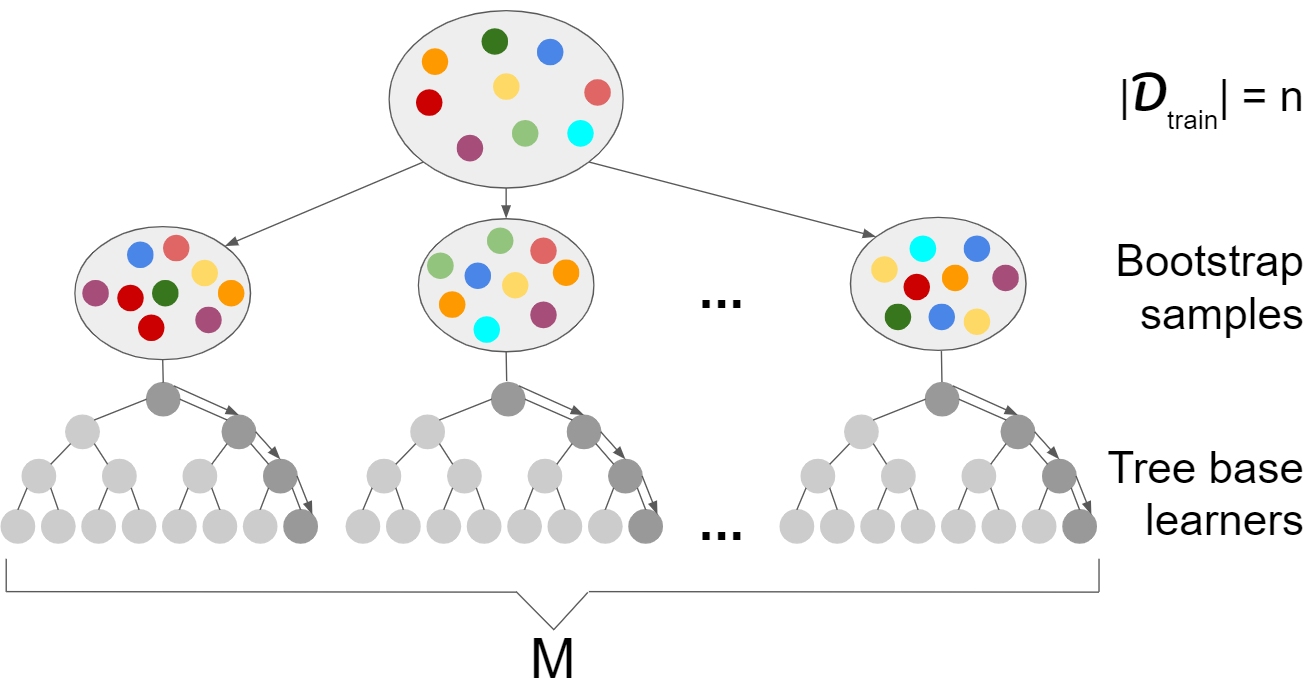
\includegraphics[width=0.6\textwidth]{figure/rf-bagging} \\
  \tiny Schematic depiction of bagging process
\end{minipage}%
\begin{minipage}[b]{0.35\textwidth}
\centering
  \includegraphics[width=0.9\textwidth]{
  ../slides/forests/figure/cart_forest_intro_3} \\
  \tiny Prediction surface for \texttt{iris} data with 500-tree ensemble
\end{minipage}

\end{frame}

% ------------------------------------------------------------------------------

\begin{frame}{Random Forests -- method summary}

\highlight{Empirical risk}

\begin{itemize}
  \item Applicable with \textbf{any} kind of loss function (just like tree base 
  learners)
  \item Computation of empirical risk for all potential child nodes in all trees
\end{itemize}

\medskip

\highlight{Optimization} ~~
\textbf{Exhaustive} search over all split candidates in each node of each tree
to minimize empirical risk in child nodes (greedy optimization) \\

\medskip

\highlight{Hyperparameters}

\begin{itemize}
  \item \textbf{Ensemble size}, i.e., number of trees
  \item \textbf{Complexity} of base learners
  \item \textbf{Number of split candidates}, i.e., number of features to be
  considered at each split \\
  $\Rightarrow$ frequently used heuristics with total of $p$ features: 
  $\left \lfloor{\sqrt{p}}\right \rfloor$ for classification,
  $\left \lfloor{p/3}\right \rfloor$ for regression
\end{itemize}

\medskip

\highlight{Out-of-bag (OOB) error}
\begin{itemize}
  \item Compute ensemble prediction for observations outside individual 
  trees' bootstrap training sample \\ $\Rightarrow$ unseen test points
  \item Use resulting loss as unbiased estimate of \textbf{generalization error}
\end{itemize}

% \highlight{Runtime behavior} ~~
% $\mathcal{O}(M \cdot n^2 \cdot p)$ for $M$ trees, $n$ observations and $p$ 
% features
  
\end{frame}

% ------------------------------------------------------------------------------

\begin{frame}{Random Forests -- Pro's \& Con's}

\begin{columns}[onlytextwidth]
  \begin{column}{0.5\textwidth}
    \highlight{Advantages}
    \footnotesize
    \begin{itemize}
      \positem Translation of most of \textbf{trees'} advantages (e.g., 
      feature selection, feature interactions)
      \positem Fairly good \textbf{good predictors}: mitigating base learners' 
      weakness through bagging
      \positem Quite \textbf{stable} w.r.t. changes in data
      \positem Good with \textbf{high-dimensional} data, even in presence of 
      noisy covariates
      % \positem Applicable to \textbf{unbalanced} data
      \positem Easy to \textbf{parallelize}
      \positem Rather easy to \textbf{tune}
      \positem Intuitive measures of \textbf{feature importance}
    \end{itemize}
  \end{column}
  \begin{column}{0.5\textwidth}
    \highlight{Disadvantages}
    \footnotesize
    \begin{itemize}
      \negitem Loss of individual trees' \textbf{interpretability} -- at least, 
      for large ensembles
      \negitem Hard to \textbf{visualize}
      \negitem Often suboptimal for \textbf{regression}
      \negitem \textbf{Bias} toward features with many categories
      \negitem Often still inferior in \textbf{performance} to other methods 
      (e.g., boosting)
    \end{itemize}
  \end{column}
\end{columns}

\vfill

\small

\conclbox{Fairly good and stable predictor with built-in feature selection, but 
black-box method}

\end{frame}

% ------------------------------------------------------------------------------

\begin{frame}{Random Forests -- Practical hints}

\highlight{Pre-processing} ~~ Inherent feature selection, but high 
\textbf{computational cost} for large number of features \\
$\Rightarrow$ upstream feature selection (e.g., via PCA) might be advisable

\medskip

\highlight{Feature importance}

\begin{itemize}
  \item Based on \textbf{improvement in split criterion:} aggregate improvements 
  by all splits using $j$-th feature
  \item Based on \textbf{permutation:} permute $j$-th feature in 
  OOB observations and compute impact on OOB error
\end{itemize}

\medskip

\highlight{Tuning} ~~ Number of split candidates often more impactful than 
number of trees

\medskip

\highlight{Implementation}

\begin{itemize}
  \item \textbf{R:} \texttt{mlr3} learners \texttt{LearnerClassifRanger} / 
    \texttt{LearnerRegrRanger}, calling \texttt{ranger::ranger()}
  \item \textbf{Python:} \texttt{RandomForestClassifier} / 
  \texttt{RandomForestRegressor} from package \texttt{scikit-learn}
\end{itemize}

\end{frame}